\newpage
\lecture{8}{Измеримая оболочка и ядро.}

\subsection{Свойства.}

\begin{definition}
    Пусть $\nu:\ \CP(X)\to[0,\, +\infty]$~--- внешняя мера. Пусть $A\subset X$. Пусть множества $K,\, E\in\CA_{\nu}$ таковы, что
    $K\subset A\subset E$. Тогда
    \begin{enumerate}
        \item если $\forall B\subset A\setminus K$ из $B\in\CA_{\nu}$ следует, что $\nu(B)=0$, то $K$ называется
              \mdef{измеримым ядром} множества $A$;
        \item если $\forall B\subset E\setminus A$ из $B\in\CA_{\nu}$ следует, что $\nu(B)=0$, то $E$ называется
              \mdef{измеримой оболочкой} множества $A$.
    \end{enumerate}

    Проще говоря, между множеством и ядром (и между множеством и оболочкой) не должно быть <<большого зазора>>, то есть мера любого измеримого
    множества $B$ (смотри рисунок \ref{fig:ker}) должна быть нулевой.
\end{definition}

\begin{figure}[!ht]
    \centering
    

\tikzset{every picture/.style={line width=0.75pt}} %set default line width to 0.75pt        

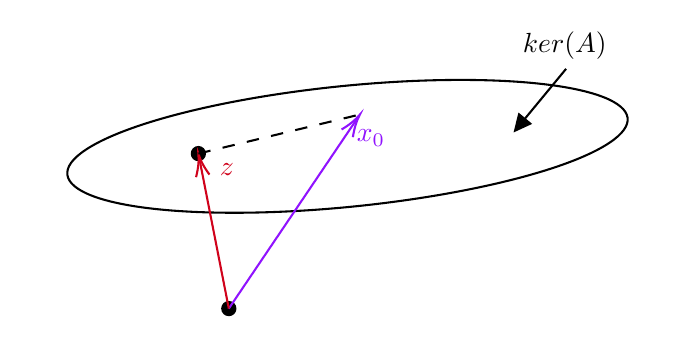
\begin{tikzpicture}[x=0.75pt,y=0.75pt,yscale=-1,xscale=1]
%uncomment if require: \path (0,300); %set diagram left start at 0, and has height of 300

%Shape: Ellipse [id:dp7555518550305362] 
\draw   (22.21,101.67) .. controls (52.33,83.99) and (132.02,69.67) .. (200.21,69.67) .. controls (268.39,69.67) and (299.25,83.99) .. (269.13,101.67) .. controls (239,119.34) and (159.31,133.67) .. (91.13,133.67) .. controls (22.94,133.67) and (-7.91,119.34) .. (22.21,101.67) -- cycle ;
%Straight Lines [id:da8611871472064767] 
\draw    (251,64.33) -- (227.58,92.69) ;
\draw [shift={(225.67,95)}, rotate = 309.56] [fill={rgb, 255:red, 0; green, 0; blue, 0 }  ][line width=0.08]  [draw opacity=0] (8.93,-4.29) -- (0,0) -- (8.93,4.29) -- cycle    ;
%Flowchart: Connector [id:dp3708456265538911] 
\draw  [fill={rgb, 255:red, 0; green, 0; blue, 0 }  ,fill opacity=1 ] (70.67,105.17) .. controls (70.67,103.42) and (72.08,102) .. (73.83,102) .. controls (75.58,102) and (77,103.42) .. (77,105.17) .. controls (77,106.92) and (75.58,108.33) .. (73.83,108.33) .. controls (72.08,108.33) and (70.67,106.92) .. (70.67,105.17) -- cycle ;
%Flowchart: Connector [id:dp6480582811904614] 
\draw  [fill={rgb, 255:red, 0; green, 0; blue, 0 }  ,fill opacity=1 ] (85.33,179.83) .. controls (85.33,178.08) and (86.75,176.67) .. (88.5,176.67) .. controls (90.25,176.67) and (91.67,178.08) .. (91.67,179.83) .. controls (91.67,181.58) and (90.25,183) .. (88.5,183) .. controls (86.75,183) and (85.33,181.58) .. (85.33,179.83) -- cycle ;
%Straight Lines [id:da2615434521627906] 
\draw [color={rgb, 255:red, 144; green, 19; blue, 254 }  ,draw opacity=1 ]   (88.5,179.83) -- (150.55,87.99) ;
\draw [shift={(151.67,86.33)}, rotate = 484.04] [color={rgb, 255:red, 144; green, 19; blue, 254 }  ,draw opacity=1 ][line width=0.75]    (10.93,-3.29) .. controls (6.95,-1.4) and (3.31,-0.3) .. (0,0) .. controls (3.31,0.3) and (6.95,1.4) .. (10.93,3.29)   ;
%Straight Lines [id:da13563403014940367] 
\draw [color={rgb, 255:red, 208; green, 2; blue, 27 }  ,draw opacity=1 ]   (74.22,107.13) -- (88.5,179.83) ;
\draw [shift={(73.83,105.17)}, rotate = 78.89] [color={rgb, 255:red, 208; green, 2; blue, 27 }  ,draw opacity=1 ][line width=0.75]    (10.93,-3.29) .. controls (6.95,-1.4) and (3.31,-0.3) .. (0,0) .. controls (3.31,0.3) and (6.95,1.4) .. (10.93,3.29)   ;
%Straight Lines [id:da7842292979954639] 
\draw  [dash pattern={on 4.5pt off 4.5pt}]  (73.83,105.17) -- (151.67,86.33) ;

% Text Node
\draw (228.67,45) node [anchor=north west][inner sep=0.75pt]   [align=left] {$\displaystyle \operatorname{ker}( A)$};
% Text Node
\draw (148.67,92.33) node [anchor=north west][inner sep=0.75pt]  [color={rgb, 255:red, 144; green, 19; blue, 254 }  ,opacity=1 ] [align=left] {$\displaystyle x_{0}$};
% Text Node
\draw (82.67,108.33) node [anchor=north west][inner sep=0.75pt]  [color={rgb, 255:red, 208; green, 2; blue, 27 }  ,opacity=1 ] [align=left] {$\displaystyle z$};


\end{tikzpicture}

    \caption{Ядро и оболочка.}
    \label{fig:ker}
\end{figure}

\begin{remark}
    $E$ является измеримой оболочкой множества $A$ тогда и только тогда, когда $E^C$ является измеримым ядром множества $A^C$.
\end{remark}

\begin{claim}
    Если $K_1,\, K_2$~--- измеримые ядра $A\subset X$, то $\nu(K_1\bigtriangleup K_2)=0$ (и аналогично для измеримых оболочек).
\end{claim}

\begin{claim}
    \label{lect8:cl:1}
    Пусть $E,\, K\in\CA_{\nu}$~--- соответственно измеримые оболочка и ядро множества $A\subset X$. Тогда
    $A\in\CA_{\nu}\Longleftrightarrow \nu(E\setminus K)=0$.

    \begin{proof}

        \circled{$\Rightarrow$} Рассмотрим $T=E\setminus K$, тогда $\nu(T)=\nu(T\cap A)+\nu(T\setminus A)$. Распишем подробнее каждое слагаемое:
        \[
            \nu(T\cap A)=\nu(\underbrace{E\cap A\setminus K}_{B\subset A\setminus K,\, B\in\CA_{\nu}}) = 0
        \]
        ~--- по определению измеримого ядра.
        Аналогично,
        \[
            \nu(T\setminus A)=\nu((E\setminus K)\cap A^C)=\nu(E\cap K^C\cap A^C)=\nu(\underbrace{(E\setminus A)\setminus K}_{B\subset E\setminus A,\, B\in\CA_{\nu}})=0
        \]
        ~--- по определению измеримой оболочки.
        Итак, получили $\nu(T)=0$.

        \circled{$\Leftarrow$} Пусть $\nu(E\setminus K)=0$. Докажем, что $\forall T\subset X$ выполняется, что $\nu(T)=\nu(T\cap A)+\nu(T\cap A^C)$.
        Заметим, что
        \begin{align*}
            \nu(T\cap A)   & \leqslant \nu(T\cap E)   \\
            \nu(T\cap A^C) & \leqslant \nu(T\cap K^C)
        \end{align*}
        Тогда
        \[
            \nu(T\cap A)+\nu(T\cap A^C)\leqslant \nu(T\cap E)+\nu(T\cap K^C).
        \]
        Далее в силу $K\subset E$:
        \[
            \nu(T\cap E)\leqslant\nu(T\cap K)+\nu(T\cap (E\setminus K))\leqslant\nu(T\cap K)+\underbrace{\nu(E\setminus K)}_{0}.
        \]
        Тогда, продолжая неравенство выше:
        \[
            \nu(T\cap A)+\nu(T\cap A^C)\leqslant \nu(T\cap E)+\nu(T\cap K^C)\leqslant \nu(T\cap K)+\nu(T\cap K^C) \underbrace{=}_{K\in\CA_{\nu}} \nu(T).
        \]


    \end{proof}
\end{claim}

\begin{remark}
    Для любых измеримых ядер $K_1,\, K_2$ множества $A$ верно, что $\nu(K_1)=\nu(K_2)$. Аналогично для измеримых оболочек.
\end{remark}

\begin{exercise}
    Пусть $X=\{1,\, 2,\, 3\}$. Возьмем меру следующим образом:
    \[
        \nu(A)=\begin{cases}
            0,\ A=\varnothing, \\
            2,\ A=X,           \\
            1,\ \text{иначе.}
        \end{cases}
    \]
    Можно проверить, что $\nu$~--- внешняя мера. Понятно, что $\CA_{\nu}=\{\varnothing,\, X\}$. Следовательно
    $\forall A\subset X,\, A\neq \varnothing,\, A\neq X$ измеримое ядро множества $A$~--- это $\varnothing$ и измеримая оболочка~--- $X$.

    \begin{remark}
        То есть может получится так, что $\nu(A)<\nu(E)$, где $E$~--- измеримая оболочка $A$.
    \end{remark}
\end{exercise}

\begin{claim}
    \label{lect8:cl:2}
    $\forall A\subset\R^d\ m^*(A)=\lambda(E)$, где $\lambda$~--- мера Лебега, $E$~--- измеримая оболочка $A$.

    \begin{proof}

        Не уменьшая общности считаем, что $m^*(A)<+\infty$.
        По определению внешней меры Лебега, $\forall n\in\N\ \exists$ элементарное множество $A_{n}\subset\R^d:\ A\subset A_{n}$ и
        $\lambda(A_{n})<m^*(A)+\dfrac{1}{n}$.

        Рассмотрим $E=\bigcap\limits_{n=1}^{\infty}A_n$~--- измеримо по Лебегу, как счётное пересечение измеримых по Лебегу множеств.
        Теперь $A\subset A_n\ \forall n\Rightarrow A\subset E\Rightarrow m^*(A)\leqslant m^*(E)=\lambda(E)$.

        С другой стороны, $\forall n\ E\subset A_n\Rightarrow \lambda(E)\leqslant \lambda(A_n)<m^*(A)+\dfrac{1}{n}\Rightarrow\lambda(E)\leqslant m^*(A)$.

        Окончательно, $\lambda(E)=m^*(A)$.

        Покажем теперь, что $E$~--- измеримая оболочка. Во-первых, $A\subset E$ и $E\in\CA_{m^*}$. Проверим, что $\forall B\subset E\setminus A$ из
        $B\in\CA_{m^*}$ следует, что $m^*(B)=0$. Предположим противное, нашлось $B\subset E\setminus A$ такое, что $B\in\CA_{m^*}$ и $m^*(B)>0$.
        Построим противоречие на том, что меры оболочки и множества совпадают.
        Возьмем $T = A\cup B\subset E$, то есть $m^*(T)\leqslant m^*(E)$.
        Тогда \[
            m^*(T)=\underbrace{m^*(T\cap B)}_{m^*(B)}+\underbrace{m^*(T\setminus B)}_{m^*(A)}\leqslant m^*(E)\Rightarrow m^*(B)\leqslant m^*(E)-m^*(A)=0.
        \]

    \end{proof}
\end{claim}

\begin{remark}
    Аналогично доказывается, что $m^*(A)=\lambda(K)$, где $K$~--- измеримое ядро $A$, если $A$~--- \textbf{измеримо}.
\end{remark}

\begin{theorem}[внешняя регулярность меры Лебега]
    Для любого измеримого по Лебегу множества $A\subset \R^d$ выполнено
    \[
        \lambda(A)=\inf\{\lambda(U)\ \mid\ U\subset \R^d\text{~--- открыто},\, A\subset U\}=:L.
    \]

    \begin{proof}

        $\forall \varepsilon>0\ \exists$ элементарное множество $A_{\varepsilon}\subset \R^d:\ A\subset A_{\varepsilon}$ и $\lambda(A_{\varepsilon})<\lambda(A)+\varepsilon$.
        Поскольку $A_{\varepsilon}$~--- элементарное, то существуют клетки $\{K_i\}_{i=1}^{n}:\ A_{\varepsilon}=\bigsqcup\limits_{i=1}^n K_i$.
        Выберем открытые клетки $\widetilde{K}_i$ так, что $K_i\subset \widetilde{K}_i$ и $\lambda(\widetilde{K}_i\setminus K_i)<\dfrac{\varepsilon}{n}$. Тогда
        имеем $\lambda(\widetilde{K}_i)\leqslant\lambda(K_i)+\lambda(\widetilde{K}_i\setminus K_i)$.
        Теперь построим $U:=\bigcup\limits_{i=1}^n\widetilde{K}_i$~--- открытое, $A\subset U$. Сложив все неравенства получим
        \[
            \lambda(U)\leqslant \sum_{i=1}^n\lambda(\widetilde{K}_i)\leqslant\underbrace{\sum_{i=1}^n\lambda(K_i)}_{\lambda(A_{\varepsilon})}+\sum_{i=1}^n\dfrac{\varepsilon}{n}
            =\lambda(A_{\varepsilon})+\varepsilon=\lambda(A)+2\varepsilon.
        \]

        Следовательно, $L\leqslant\lambda(A)$, но $A\subset U\Rightarrow\lambda(U)\geqslant\lambda(A)\Rightarrow L\geqslant \lambda(A)$, поэтому $L=\lambda(A)$.

    \end{proof}
\end{theorem}

Аналогично можно показать, что выполнена и следующая теорема.

\begin{theorem}[внутренняя регулярность меры Лебега]
    Для любого измеримого по Лебегу множества $A\subset \R^d$ выполнено
    \[
        \lambda(A)=\sup\{\lambda(F)\ \mid\ F\subset A\text{~--- замкнуто}\}=\sup\{\lambda(K)\ \mid\ K\subset A\text{~--- компакт}\}.
    \]
\end{theorem}

\begin{remark}
    Из доказательства утверждения \ref{lect8:cl:2} видно, что $\forall A\subset \R^d$ с конечной внешней мерой Лебега: $m^*(A)<+\infty$ существует
    борелевское множество $E\subset\R^d$, являющееся измеримой оболочкой множества $A$.

    \begin{enumerate}
        \item Если $A$~--- измеримо по Лебегу, то $\lambda(E\setminus A)=0$. То есть измеримое по Лебегу множество можно представить в виде борелевского множества и
              множества меры нуль:
              \[
                  A = \underbrace{E}_{\CB(\R^d)}\setminus \overbrace{(E\setminus A)}^{\lambda = 0}.
              \]
        \item Также существует борелевское множество $K\in\CB(\R^d)$ и $N\subset\R^d:\ A=K\sqcup N$ и $m^*(N)=0$.
              В самом деле, в силу внутренней регулярности $\lambda$ имеем $\forall n\in\N\ \exists$ замкнутое $F_n\subset A:\ \lambda(F_n)>\lambda(A)-\dfrac{1}{n}$.
              Тогда можем взять $K:=\bigcup\limits_{n=1}^{\infty}F_n$ и $N:=A\setminus K$.
        \item И верно обратное, то есть, если $A=K\sqcup N$, где $K\in\CB(\R^d)$ и $m^*(N)=0$, то $A$~--- измеримо по Лебегу.
    \end{enumerate}
\end{remark}